\documentclass{article}
\usepackage[section]{placeins}
\usepackage{graphicx, wrapfig, amsmath, amssymb, physics, hyperref}
\hypersetup{
    colorlinks=true,
    linkcolor=blue,
    filecolor=magenta,      
    urlcolor=cyan,
    }

\author{Yaghoub Shahmari}
\title{Report - Problem Set No 5}
\date{\today}
\graphicspath{ {../Figs/} }

\begin{document}
    \maketitle
    \section*{Problem 1}
    \textbf{Basic description:}

    In this problem, we're going to discuss 2D Random Walkers.
    As the lecture notes described, we expect our results to show these relations:

    \begin{gather*}
        \langle r^{2}\rangle =2dDt,D=\dfrac{l^{2}}{2dr}\\
        R_{g}=\sqrt{\langle r^{2}\rangle },\tau =l=1,d=2\\
        \Rightarrow R_{g}=\sqrt{t}
    \end{gather*}
    
    The simulation creates a list of random choices of steps
    and calculates the sum of total changes of location of the random walker.
    The number of chosen random steps is equal to $t$.
    We repeat the simulation for different $t$ many times
    and calculate the gyration radius of the all of final positions of each $t$.

    \textbf{Results:}

    \begin{figure}[!htb]
        \centering
        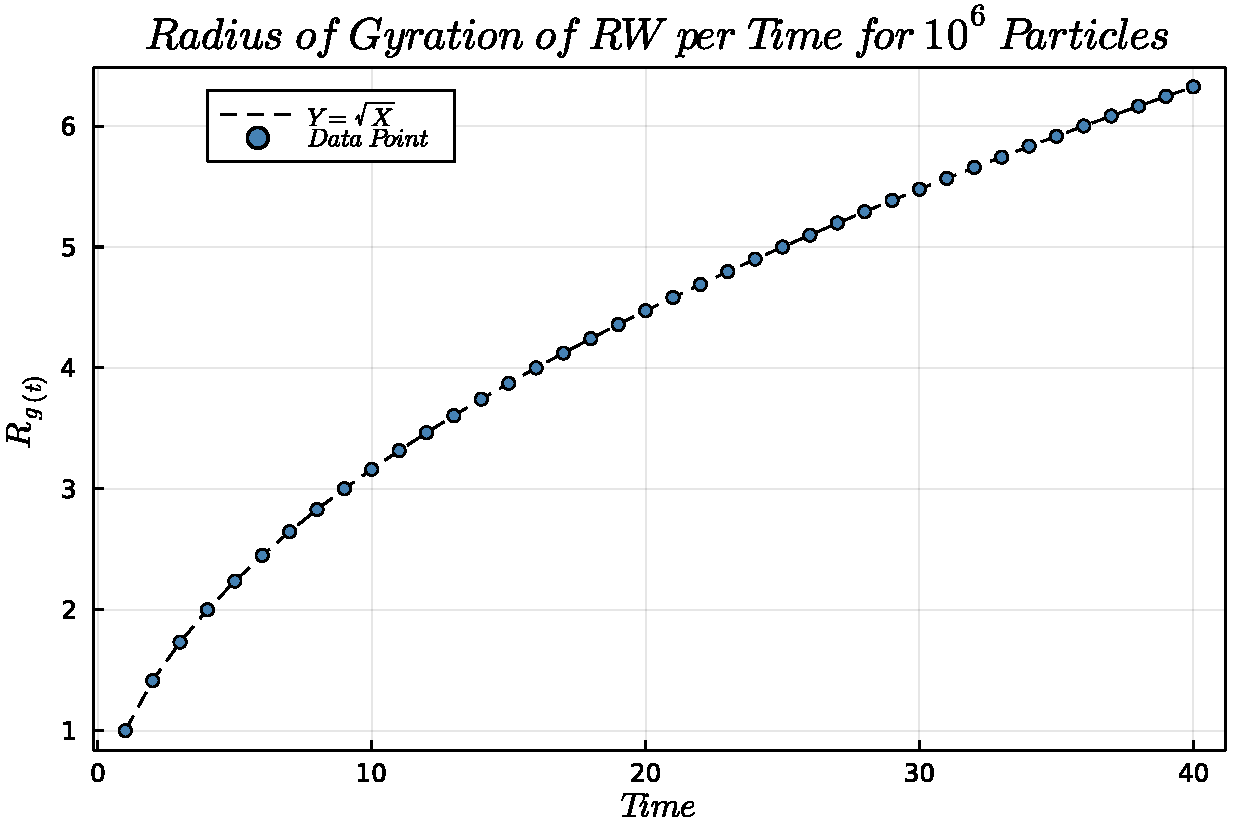
\includegraphics[scale = 0.4]{/Q1/Q1-Rg(t)}
        \label{fig:1.1}
        \caption{Gyration radius of each time step.}
    \end{figure}

    \begin{figure}[!htb]
        \centering
        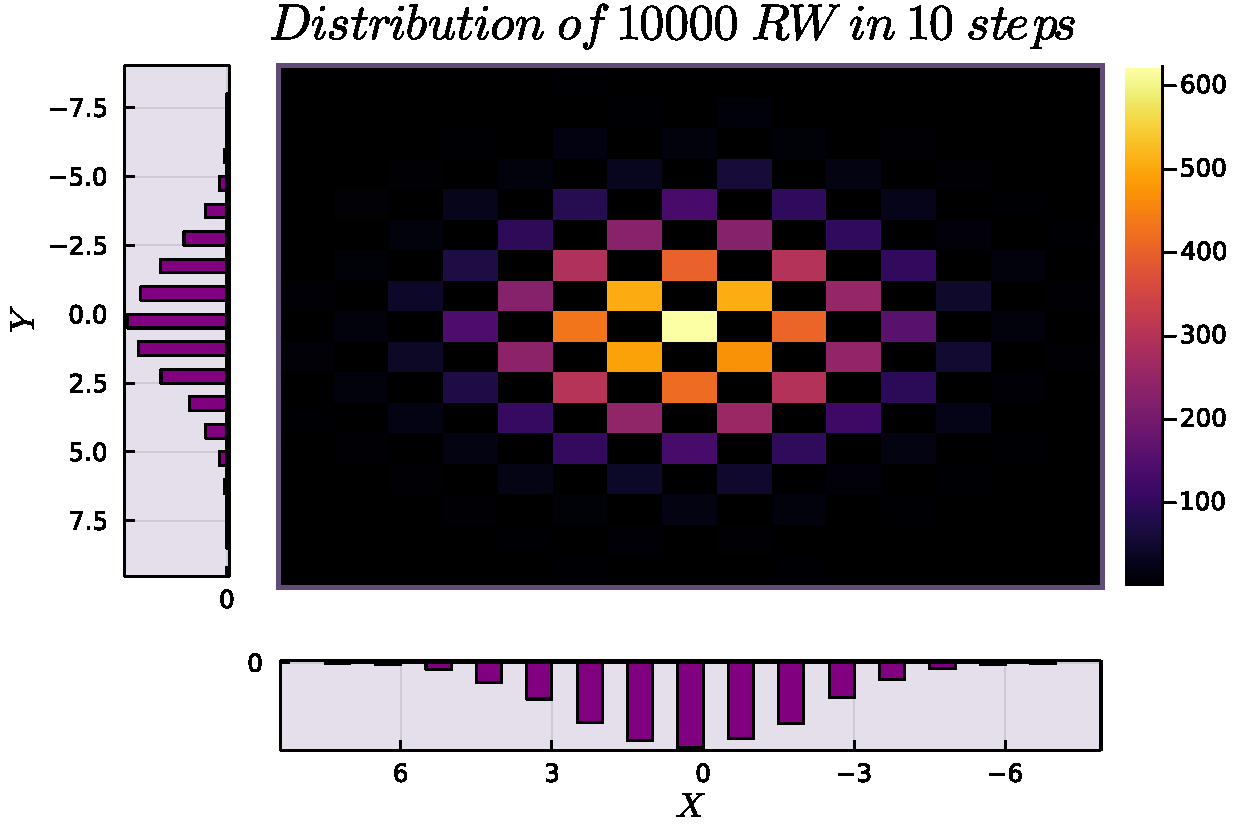
\includegraphics[scale = 0.4]{/Q1/Q1-2DHist1}
        \label{fig:1.2}
        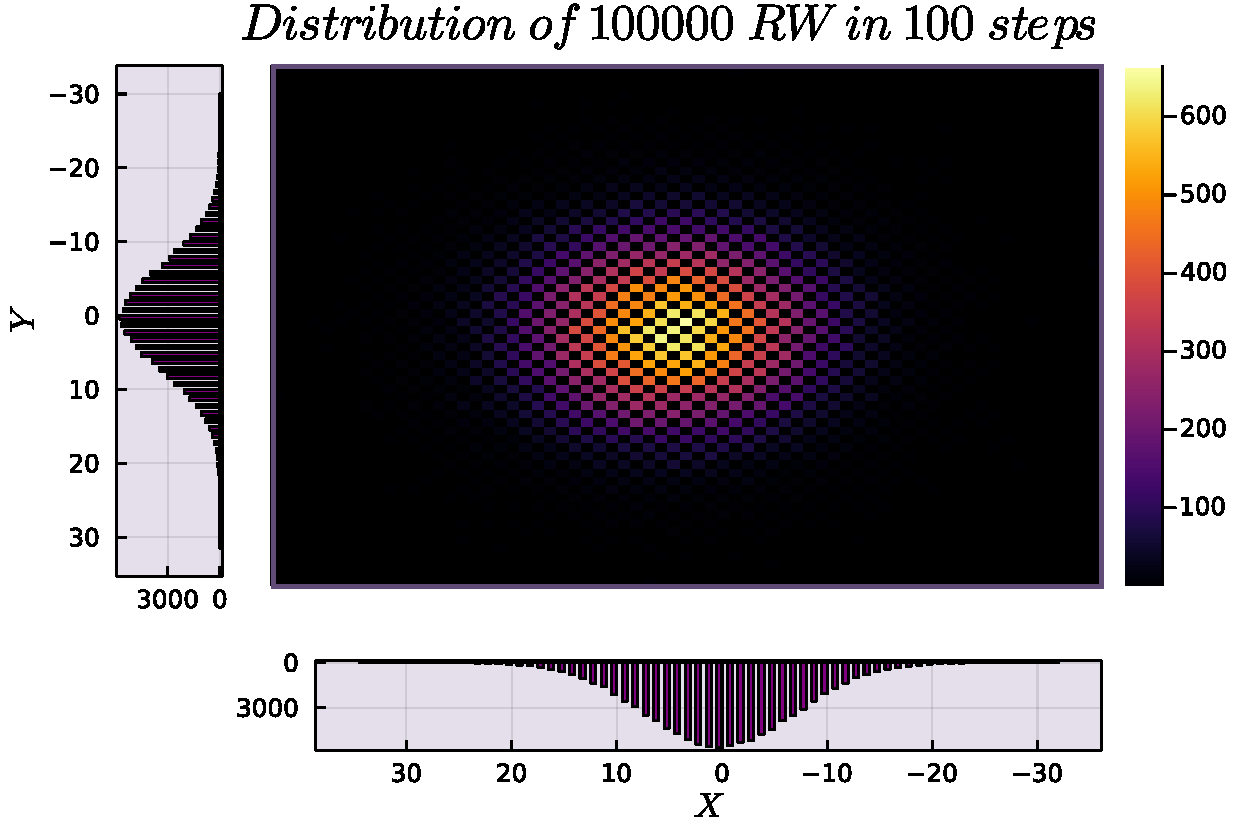
\includegraphics[scale = 0.4]{/Q1/Q1-2DHist2}
        \label{fig:1.3}
        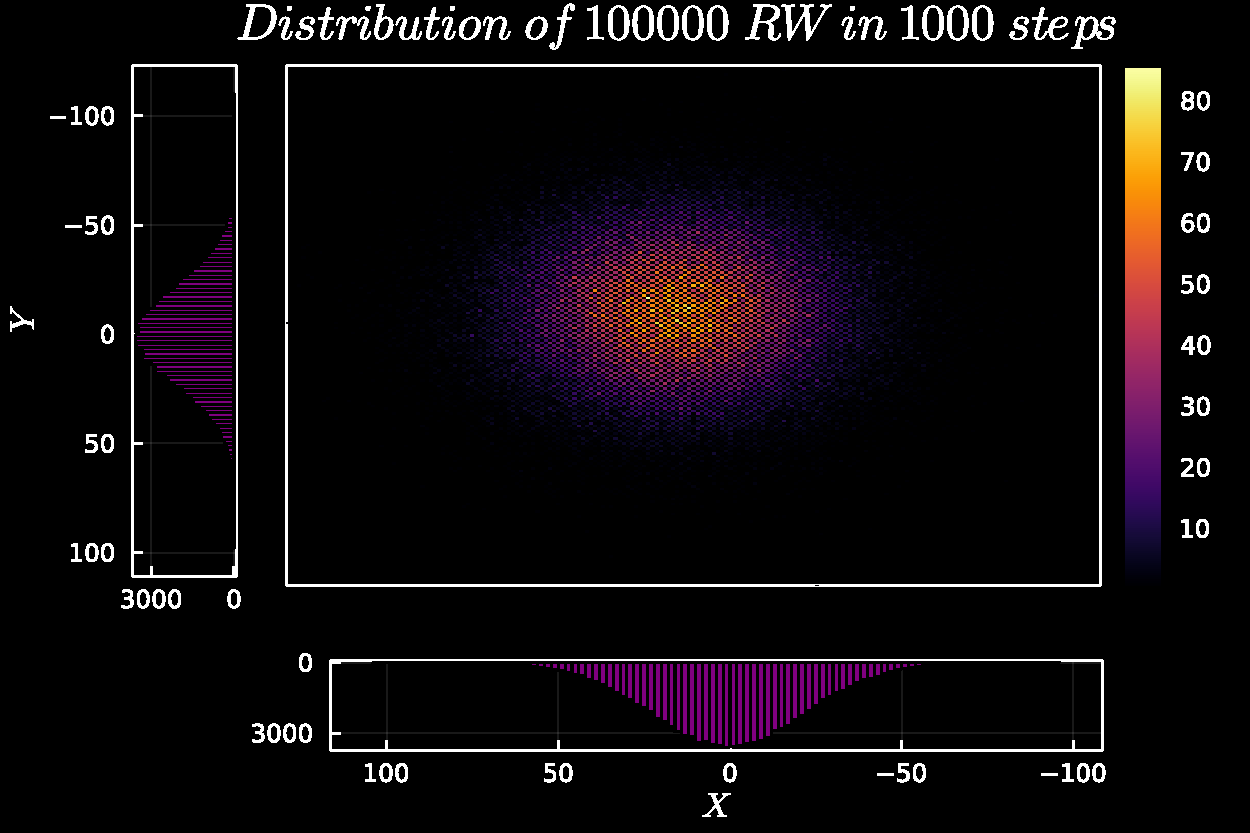
\includegraphics[scale = 0.4]{/Q1/Q1-2DHist3}
        \label{fig:1.4}
        \caption{2D Histogram, Shows distribute of Random Walkers in 10th, 100th, and 1000th time step.}
    \end{figure}

    \pagebreak

    \section*{Problem 2}
    \textbf{Basic description:}



    \centering
    \textbf{The whole data I gathered is in \href{https://github.com/shahmari/ComputationalPhysics-Fall2021/tree/main/ProblemSet4/Data}{this link}}
    
    Thanks for watching :)
\end{document}